\chapter{Anhang}
\newpage
\section{Unterschiede und Handlungsempfehlungen für die Lerntheorien in der Übersicht}
\begin{table}[h]
	\caption{Unterschiede und Handlungsempfehlungen für die Lerntheorien in der Übersicht. Eigene Darstellung, basierend auf den Inhalten dieser Arbeit.}
	\vspace{1em}
	\centering
	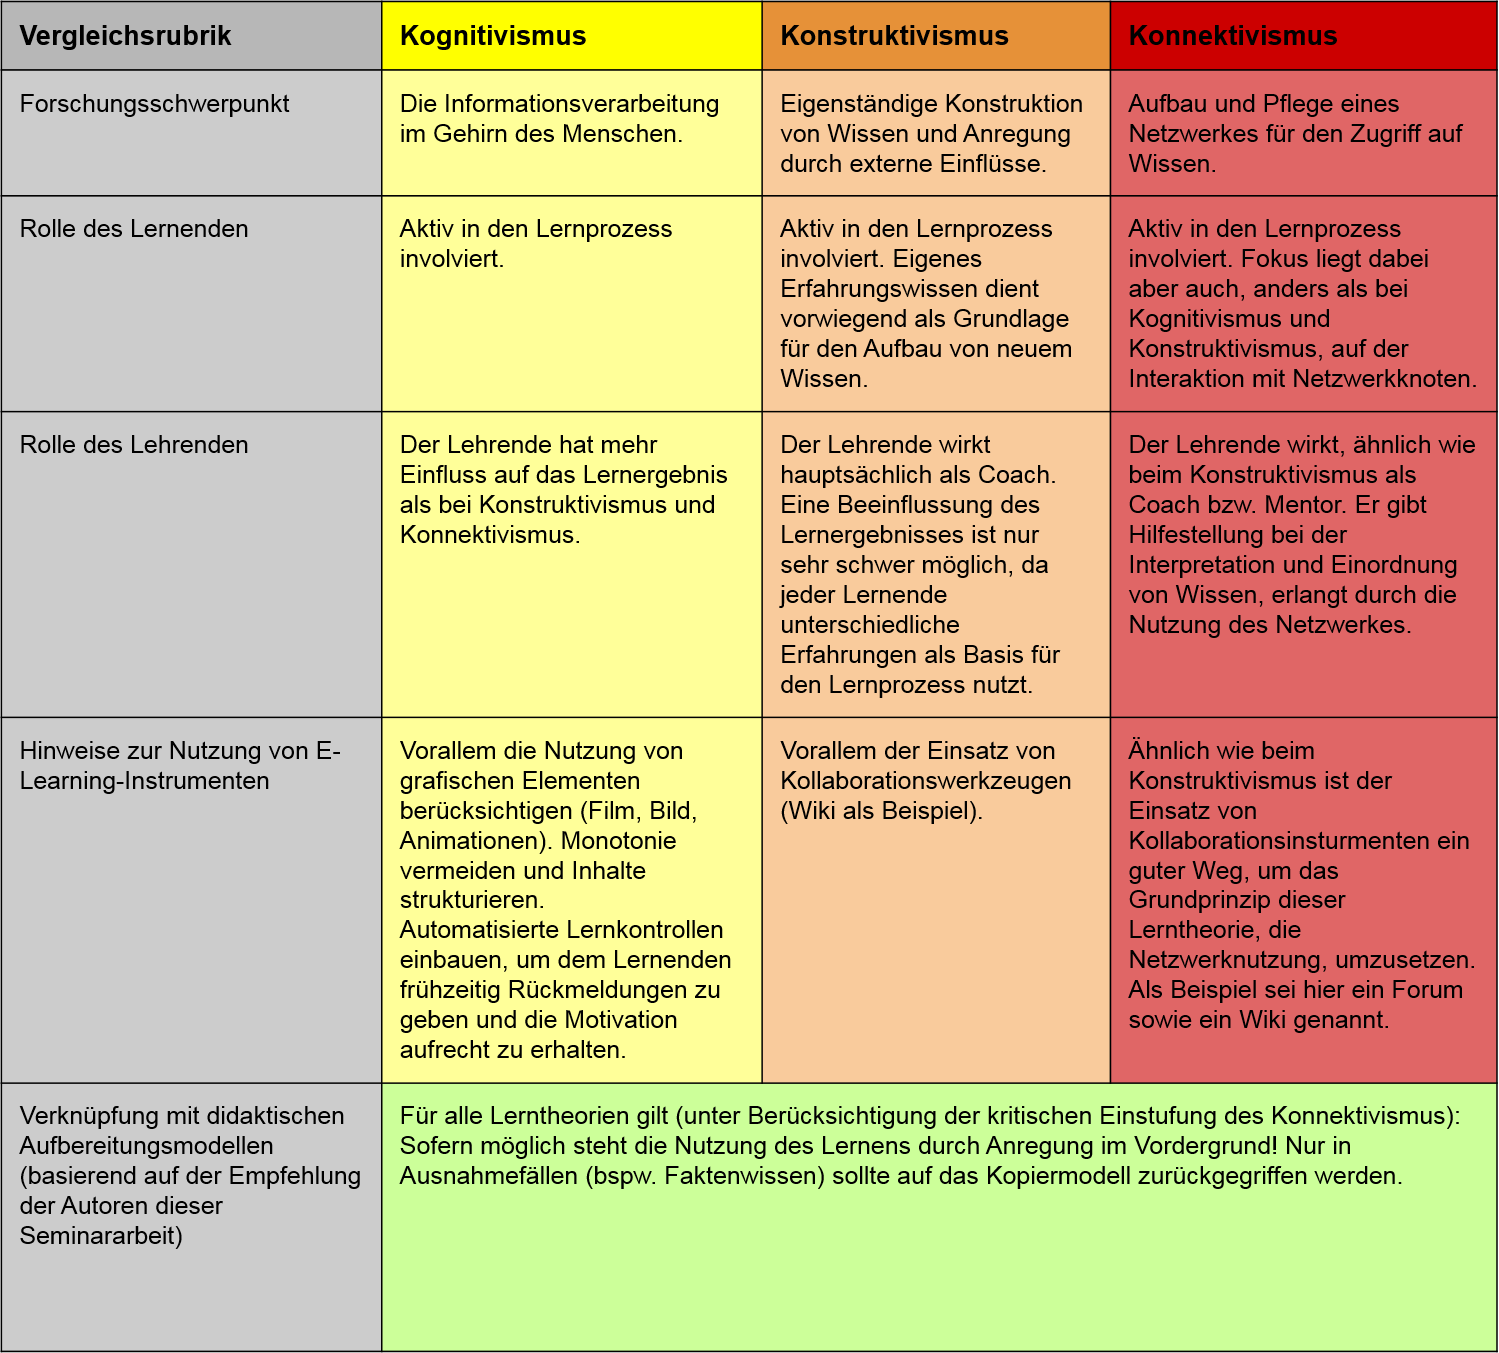
\includegraphics[width=1.0\textwidth]{Abbildungen/Gegenuberstellung.png}
	
	\label{fig:Unterschiede und Handlungsempfehlungen für die Lerntheorien}
\end{table}